% !TEX root = ../../ThesisGchatzi.tex

\subsection{Problem Definition}
\label{subsec:local_sim_join_problem}

\graphicspath{{Papers/SSTD2019/}{Papers/SIGSpatial2019/}}

We consider a set of {\em co-evolving} time series, so all time series are {\em time-aligned} and each series has a value at each of the $k$ timestamps. Given a set of such co-evolving time series, our goal is to find {\em pairs} of time series that have similar values locally over some time intervals of significant duration. More specifically:

\begin{mydefinition}[Locally Similar Time Series]
Two co-evolving time series $Τ_i$ and $Τ_j$ are locally similar if there exists a time interval $I$ spanning at least $\delta$ consecutive timestamps such that at every timestamp in $I$ their corresponding values do not differ by more than a given threshold $\epsilon$, i.e., $\forall t \in I, |T_i.v_t - T_j.v_t| \leq \epsilon$.
\end{mydefinition}

Note that threshold $\epsilon$ expresses the maximum tolerable deviation per timestamp between two time series, so it actually concerns the absolute difference of their corresponding values. We wish to find all such pairs of time series, so the problem is actually a {\em self-join} over the dataset, specifying as join criteria the distance threshold $\epsilon$ and the minimum time duration $\delta$ of qualifying pairs. More formally:

\begin{problem}[Pair Discovery over Time Series]
Given a set of $r$ co-evolving time series $\mathcal{T}=\{T_1,T_2,...,T_r\}$ of equal duration $n$, a distance threshold $\epsilon>0$, and a time duration threshold $\delta>1$ timestamps, $(\delta \in N)$, retrieve all pairs $\{T_i, T_j\}, 1 \leq i < j \leq r$ of locally similar time series along with the corresponding time intervals.
\end{problem}

For example, in Figure~\ref{fig:sim_join}, the detected pairs for specified $\epsilon$ and $\delta$ would be the locally similar time series within grey ribbons. Since two time series might be locally similar in more than one intervals, their matching subsequences are considered as two different pairs, one for each interval. For instance, in Figure~\ref{fig:sim_join} the green and red time series yield two matching pairs in different time intervals.

\begin{figure}[!tb]
    \centering
    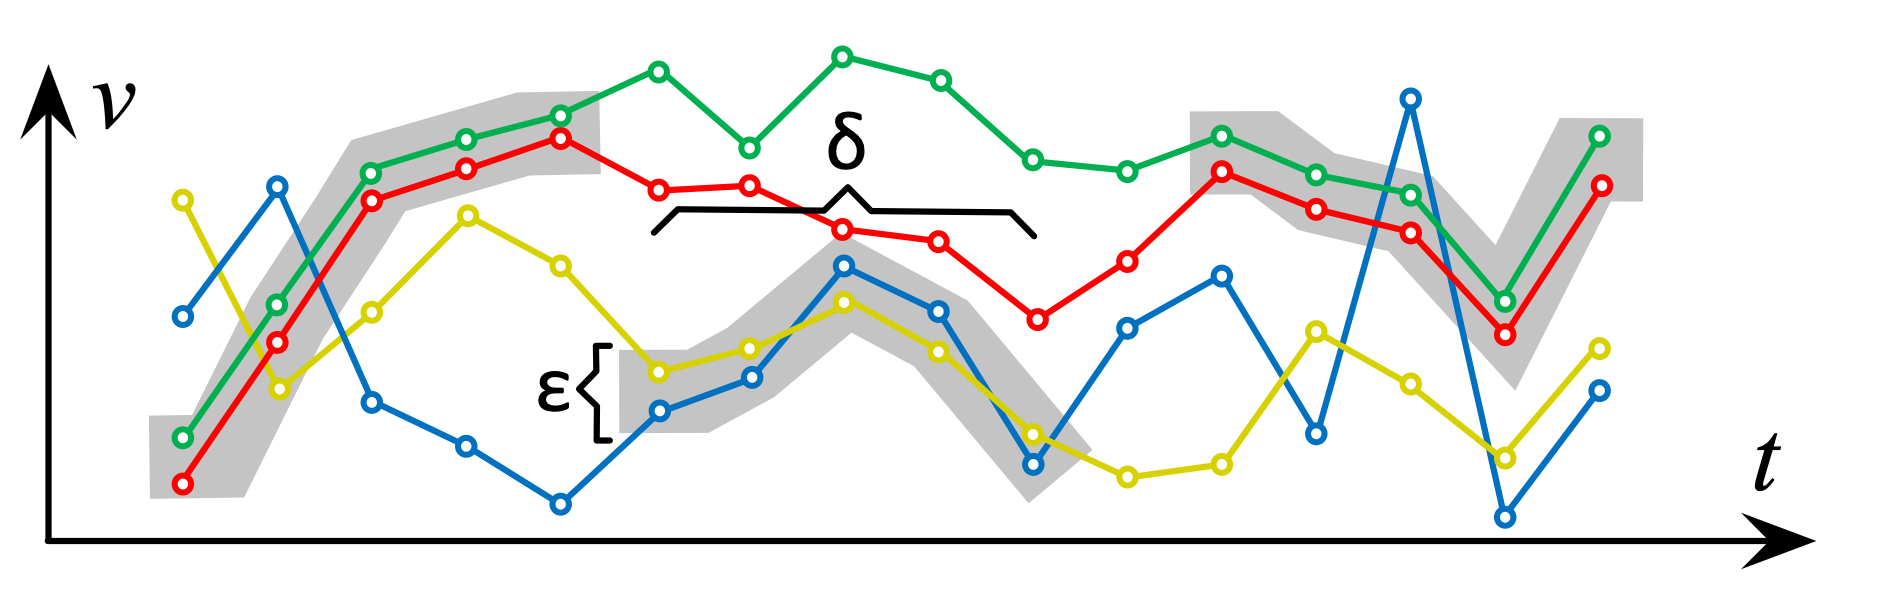
\includegraphics[width=0.55\textwidth]{figures/sim_join.png}
    \caption{Pair discovery over a set of time series.}
    \label{fig:sim_join}
\end{figure}

The above problem can be extended to the detection of groups, called \textit{bundles}, of co-evolving time series. Each such bundle of time series contains at least a pre-defined number $\mu>2$ of members, which are pairwise locally similar to each other over a time interval of sufficient duration. This problem can be formulated as follows:

\begin{problem}[Local Bundle Discovery over Time Series]
Given a set of co-evolving time series $\mathcal{T}=\{T_1,T_2,...,T_r\}$ of equal length $n$, a minimum bundle size $\mu > 2, (\mu \in \mathbb{N}$), a maximum value difference $\epsilon>0$, and a minimum time duration $\delta>1$ timestamps, $(\delta \in \mathbb{N})$, retrieve all groups $\mathcal{G}$ of time series such that:
\begin{itemize}
    \item Each group $G \in \mathcal{G}$ contains at least $\mu$ time series.
    \item Within each group $G \in \mathcal{G}$, all pairs of time series are locally similar with respect to $\epsilon$ and $\delta$.
    \item Each group $G \in \mathcal{G}$ is \textit{maximal}, i.e., there is no other group $G' \supseteq G$ that also forms a bundle for the same time interval. 
\end{itemize}
\end{problem}

An illustration of the above problem is shown in Figure \ref{fig:bundle_disc}. Each grey band covers the subsequences of at least $\mu=3$ time series that constitute a bundle. These subsequences are pairwise locally similar for a specified distance $\epsilon$ and duration $\delta$.

\begin{figure}[!tb]
    \centering
    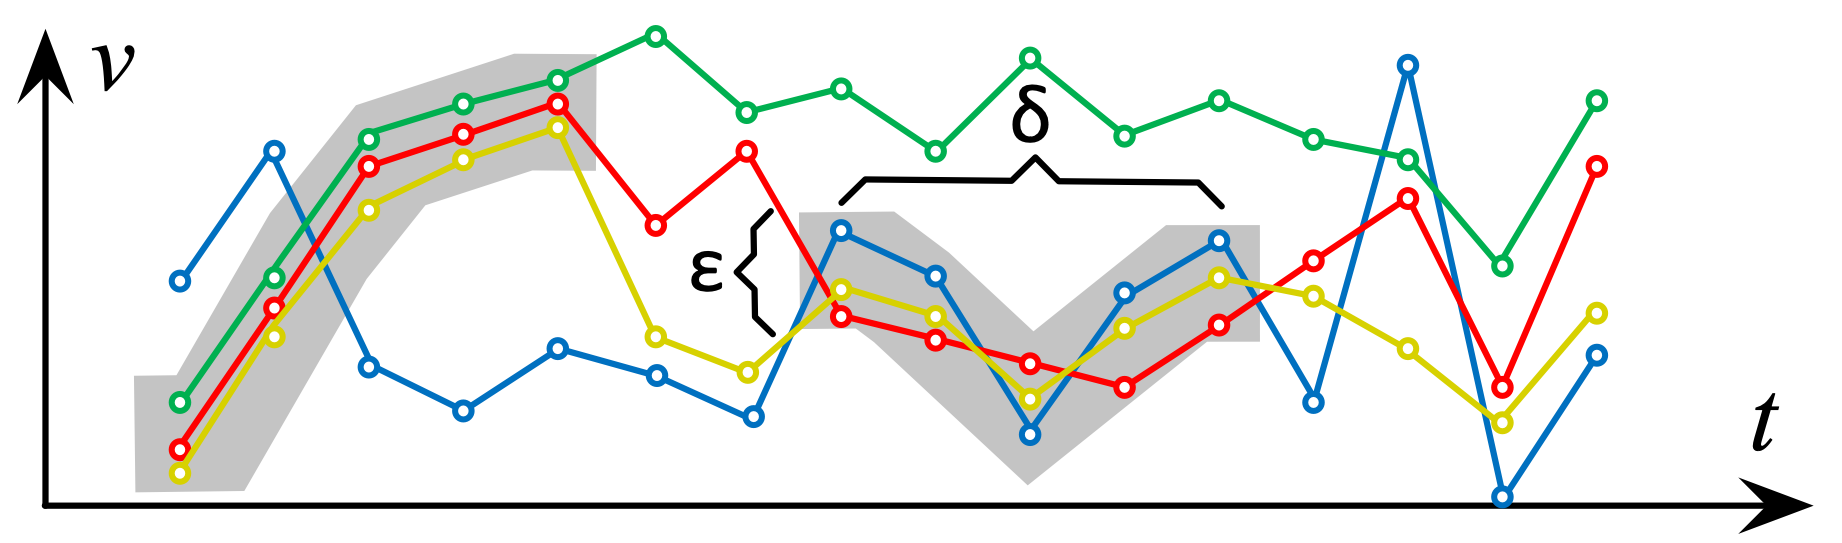
\includegraphics[width=0.55\textwidth]{figures/bundle_disc.png}
    \caption{Bundle discovery over a set of time series.}
    \label{fig:bundle_disc}
\end{figure}